\chapter{Implementación de la solución}
\label{chapter:implementacion}

\section{Clases}

Para el desarrollo de la aplicación se usó el lenguaje Python, dividiendo la aplicación en clases cuya relación puede ser vista en la figura \ref{fig:diagramaClases}. Estas clases se categorizan en: Clases visuales; clases 3D y clases de cubos.

\begin{figure}[ht]
  \centering
  \includegraphics[scale=.5]{images/diagramaClases}
  \caption{\em Diagrama de clases de la aplicación Lattice Designer.}
  \label{fig:diagramaClases}
\end{figure}

\subsection{Clases visuales}

Estas clases están relacionadas directamente con la interfaz gráfica de usuario. Permiten crear las distintas ventanas, objetos e interacciones de los usuarios con estos.

\subsubsection{LatticeDesigner}
Esta es la clase principal de la aplicación, ya que es la encargada de iniciar el programa, cargando todas las dependencias necesarias para su ejecución, pero principalmente implementa la lógica de la parte visual del \emph{software}, es decir, de la creación y distribución en pantalla de los distintos elementos visuales, como ventanas, botones, campos de texto, etc., además de la interacción del usuario con estos. Cada reacción a una acción ejecutada sobre estos elementos es orquestada por esta clase.

\subsubsection{BitmapGrid}
La clase BitmapGrid es la encargada de manejar la grilla con la cuales los científicos diseñarán las configuraciones atómicas que se simularán. Para esto se basa en la biblioteca \emph{wx.grid} de \emph{wxPython}, una implementación de una planilla de cálculos tipo \emph{excel}, la cual es modificada para no poder ser editada y que las distintas acciones del \emph{mouse} sobre esta (click, seleccionar fila o columna, seleccionar un rango de celdas, etc.) generen cambios en el color de fondo de cada celda, pudiendo este ser negro o blanco, transformando esta planilla de cálculos en un mapa de bits binario.

Entre las características de este mapa de bits se encuentra la capacidad de crear figuras predefinidas rápidamente. Por ejemplo, se puede dibujar un cuadrilátero indicando el ancho, el alto y seleccionando la esquina superior derecha de esta figura. También es posible crear un círculo indicando el radio que tendrá este y su centro. Estas dos figuras predefinidas pueden combinarse para crear configuraciones más complejas, como un elipsoide, que son de mucha utilidad para los científicos (ver figura \ref{elipsoide}).

\begin{figure}[ht]
  \centering
  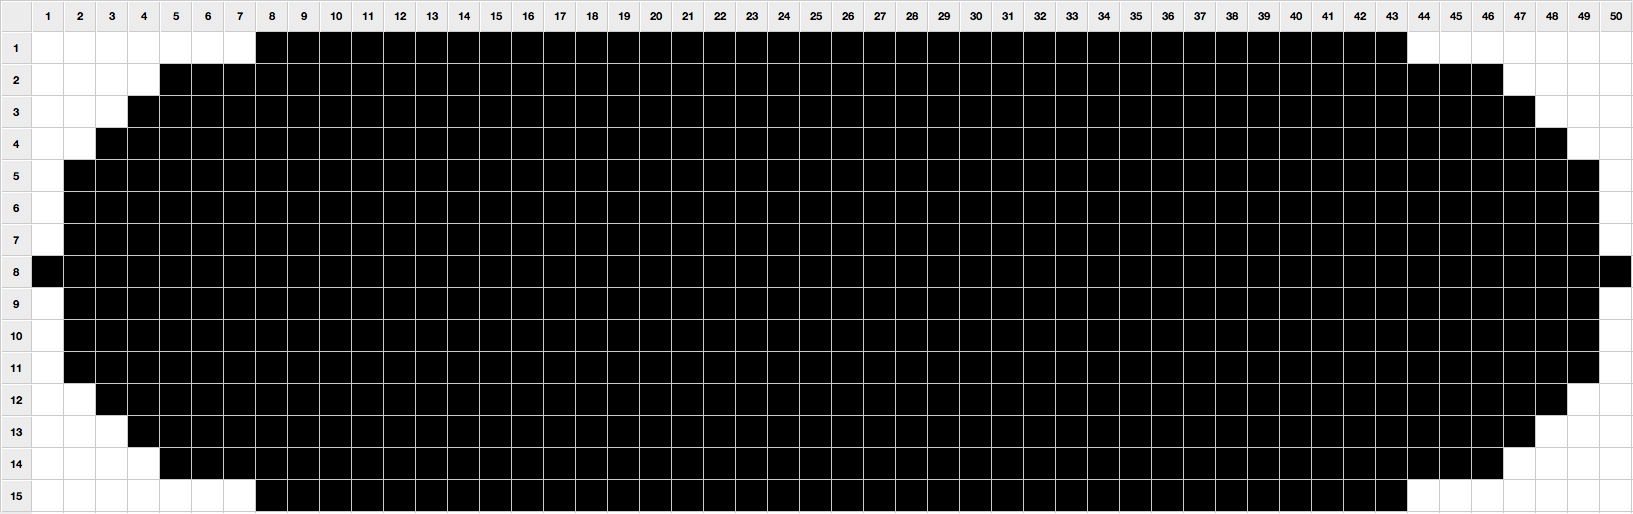
\includegraphics[scale=.25]{images/elipsoide}
  \caption{\em Mapa de bits binario con 2 figuras pre-diseñadas.}
  \label{elipsoide}
\end{figure}

\subsection{Clases 3D}

Estas clases son las encargadas de manejar los distintos \emph{canvas} que se usan en el \emph{software}, tanto para la visualización del diseño y del resultado de la simulación, como para ayudas referenciales para los científicos.

\subsubsection{AtomCanvas}

La clase AtomCanvas es la más importante con respecto a la visualización 3D, ya que es la encargada de mostrar en pantalla tanto el diseño de los objetos sobre los cuales se correrá la simulación como los resultados de estas usando OpenGL. En el desarrollo de esta clase se puso énfasis en la optimización, pudiendo mostrar sin mayores demoras más de 20.000 átomos. Para tener una idea un sistema promedio escalado analizado por los científicos usa 3.000 átomos.

Otra de las tareas de esta clase es manejar las distintas interacciones del usuario, tanto con el teclado como con el \emph{mouse} con las representaciones en 3D, como rotaciones, movimientos y \emph{zoom}.

Para la visualización del diseño se usan esferas de distintos colores, representando cada uno de los distintos tipos de átomos que pueden haber según la estructura cúbica elegida. En las figuras \ref{atomCanvas-SC}, \ref{atomCanvas-BCC} y \ref{atomCanvas-FCC} se representan una estructura de 5x5 átomos, con 3 capas, siendo diferente solo la estructura cristalina elegida.

\begin{figure}[ht]
  \centering
  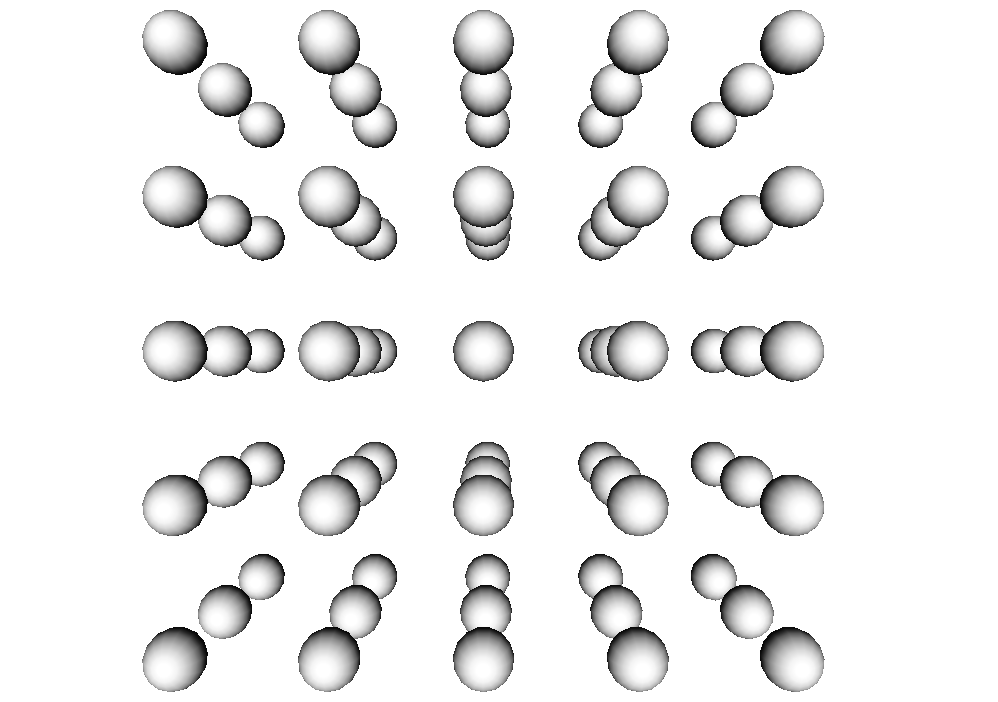
\includegraphics[scale=.3]{images/atomCanvas-SC}
  \caption{\em En un SC todos los átomos son blancos.}
  \label{atomCanvas-SC}
\end{figure}

\begin{figure}[ht]
  \centering
  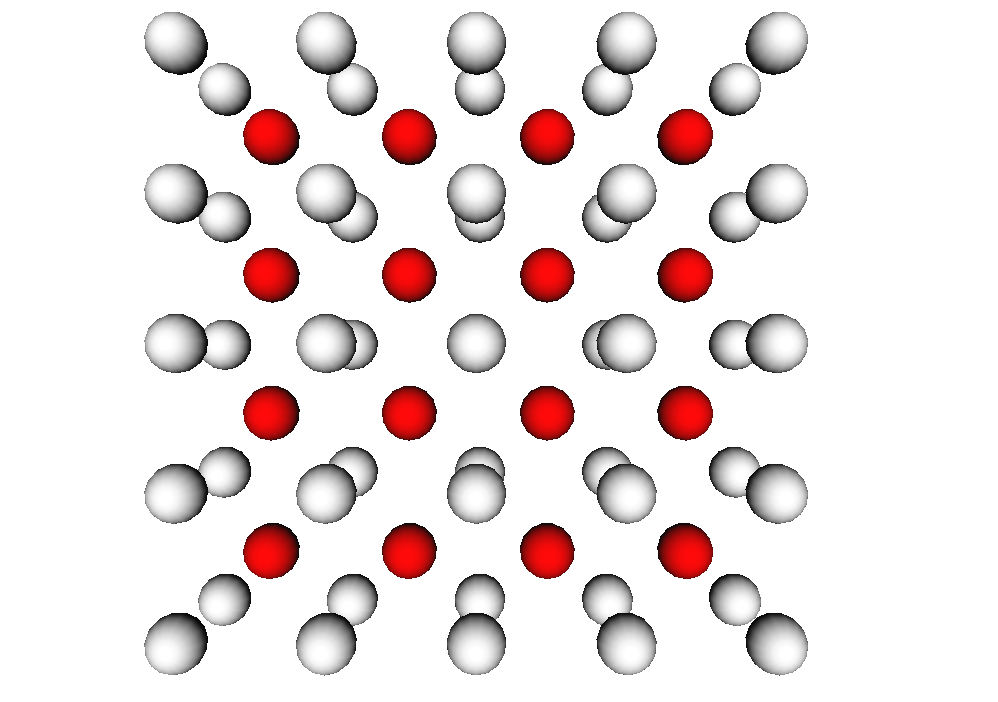
\includegraphics[scale=.3]{images/atomCanvas-BCC}
  \caption{\em En un BCC los átomos centrales son rojos.}
  \label{atomCanvas-BCC}
\end{figure}

\begin{figure}[ht]
  \centering
  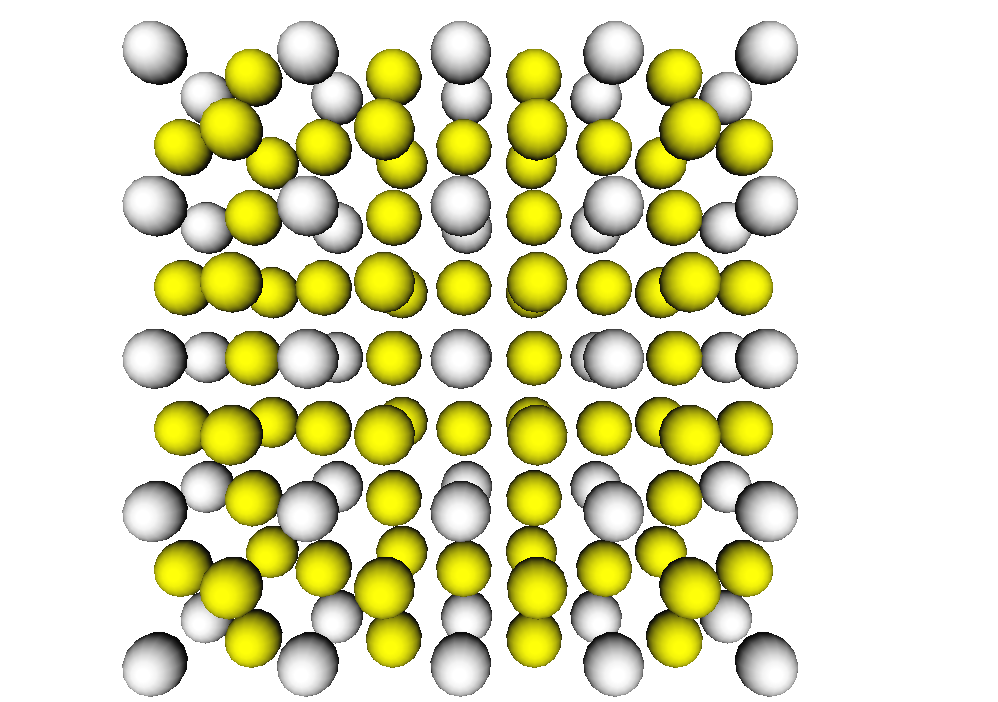
\includegraphics[scale=.35]{images/atomCanvas-FCC}
  \caption{\em En un FCC los átomos de las caras son amarillos.}
  \label{atomCanvas-FCC}
\end{figure}

En el caso de la visualización de resultados se usan flechas de colores como representación del vector de magnetización. Para asignar un color a una flecha se parte de la premisa que en tiempo t=0 el campo magnético externo está siendo aplicado hacia un eje, y por lo tanto inicialmente todos los vectores tendrán la misma magnitud, sentido y dirección, paralelos al campo externo, como se puede notar en la figura \ref{atomCanvas-vectores-inicial}. Además se sabe que en ese momento su magnitud es máxima. Si inicialmente todos los vectores son paralelos al eje A, se usa la componente â de cada vector para definir el color. Si la componente es 0 entonces será de color verde; si la magnitud es máxima en sentido contrario a los vectores iniciales el color será azul; si la magnitud es máxima en el mismo sentido de los vectores iniciales el color será rojo. Como se puede inferir la escala va desde azul a rojo, siendo este último color el inicial para todos los vectores. En la figura \ref{atomCanvas-vectores-colores} se puede ver los distintos colores según la componente $\hat{i}$ de los vectores, dado que el campo externo inicial tiene sentido $[1, 0, 0]$.

\begin{figure}[ht]
  \centering
  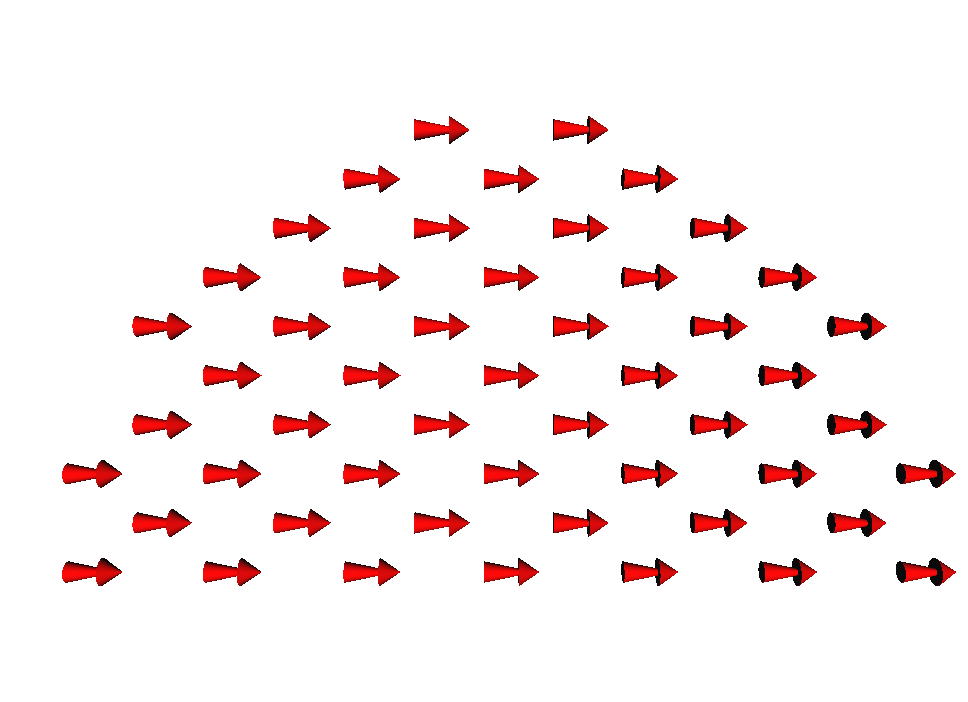
\includegraphics[scale=.3]{images/atomCanvas-vectores-inicial}
  \caption{\em Estado inicial de la visualización, con todos los vectores rojos paralelos al campo magnético externo inicial.}
  \label{atomCanvas-vectores-inicial}
\end{figure}

\begin{figure}[ht]
  \centering
  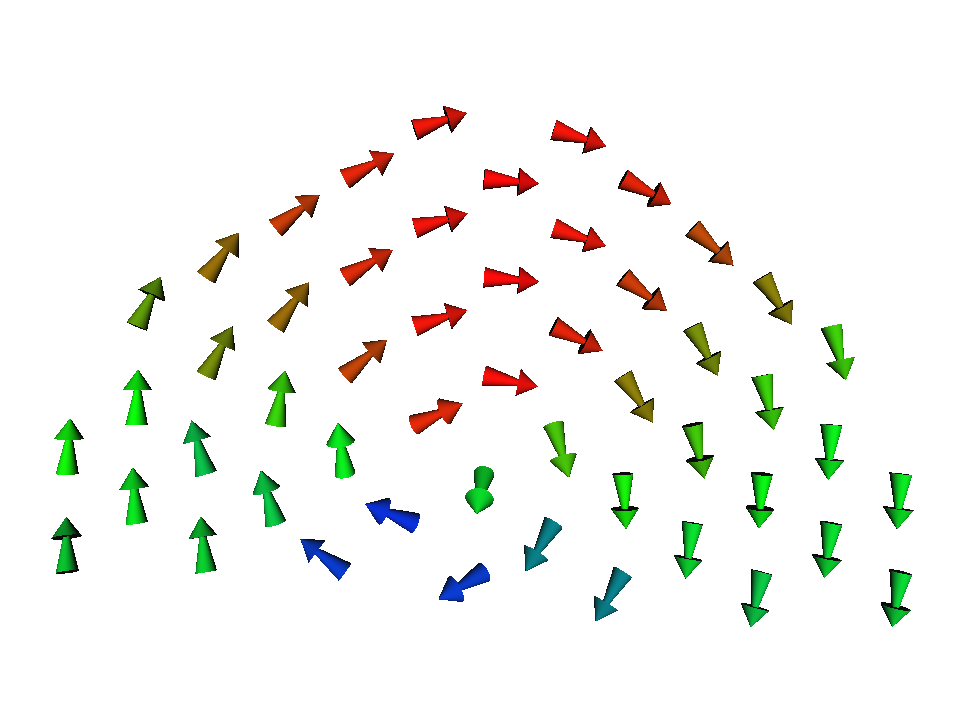
\includegraphics[scale=.3]{images/atomCanvas-vectores-colores}
  \caption{\em Vectores de distintos colores según la componente $\hat{i}$.}
  \label{atomCanvas-vectores-colores}
\end{figure}

\subsubsection{Axes}

La clase Axes es la encargada de mostrar los ejes coordenados de los distintos canvas, tanto del de diseño de objetos como el de visualización de resultados, usando Open GL.
Cada eje se representa con su propio color, usando azul, rojo y verde para los ejes X, Y y Z respectivamente, y una etiqueta con el mismo color, de forma de hacerlo fácil de visualizar para el usuario.
Debido al diseño del \emph{software}, donde las distintas funciones del programa (diseño y visualización) se seleccionan mediante pestañas, esta clase debe ser instanciada 2 veces, ya que no es posible usar la misma instancia en ambas secciones. Estas se comunican directamente con AtomCanvas para obtener los distintos parámetros de rotación de forma que los ejes sean coherentes a la imagen mostrada.

\begin{figure}[ht]
  \centering
  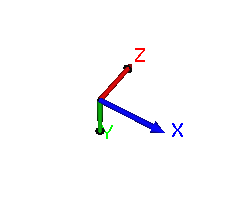
\includegraphics[scale=1]{images/axes}
  \caption{\em Representación visual de los ejes coordenados.}
\end{figure}

\subsection{Clases de cubos}


Las clases de cubos son 3 clases (\emph{SC}, \emph{BCC} y \emph{FCC}) que heredan de un mismo padre, \emph{Cube}. Estas crean los átomos de un objeto que se está diseñando. Las 3 clases hermanas tienen solo 2 métodos: \emph{calculate} y \emph{find\_neighborhood}. El primero se encarga de identificar todos los átomos que conforman la configuración atómica, dados los parámetros físicos como la estructura de la primera capa. El segundo define cuales son los parámetros para llamar al método \emph{find\_neighborhood} de la súper clase, el que busca todos los vecinos inmediatos para cada átomo. Estos parametros son necesarios para exportar el archivo que luego servirá de entrada para la simulación.

\subsubsection{Cube}
TBD


\subsubsection{SC}
\label{cubeClasesSC}
SC es la clase que maneja los cubos simples (\emph{Simple Cubic} o \emph{SC}), estas estructuras cúbicas se caracterizan por tener un átomo en cada uno de sus vértices, por lo que la identificación de sus átomos se reduce a simplemente repetir la capa superior tantas veces como sea indicado en la entrada de propiedades físicas. Para encontrar el vecindario es necesario buscar todos los átomos que estén en las siguientes posiciones relativas [-1,0,0], [1,0,0], [0,-1,0], [0,1,0], [0,0,-1] y [0,0,1], por lo que el tamaño máximo de su vecindad es de 6 átomos.

\subsubsection{BCC}
BCC es la clase que maneja los cubos centrados en el cuerpo (\emph{Body Centered Cubic} o \emph{BCC}), que son las estructuras cúbicas que además de tener un átomo en cada vértice de los cubos tienen uno en el centro de cada uno de estos. Esto implica que en la identificación de átomos se debe trabajar con una capa intermedia que contiene los centros de cada cubo. por ejemplo, para una estructura de 5 capas quedaría así:
\begin{center}
  \begin{tabular}{ c | l }
    \# & Capa \\
    \hline
    1 & Primaria \\
    2 & Intermedia \\
    3 & Primaria \\
    4 & Intermedia \\
    5 & Primaria \\
    \hline
  \end{tabular}
\end{center}

La regla para agregar un átomo central es que debe tener un cubo de átomos a su alrededor, y en caso que el cubo no esté completo simplemente se usan las capas primarias, como se puede notar en las figuras \ref{BCC-incomplete-molecule} y \ref{BCC-complete-molecule}.

\begin{figure}[ht]
  \centering
  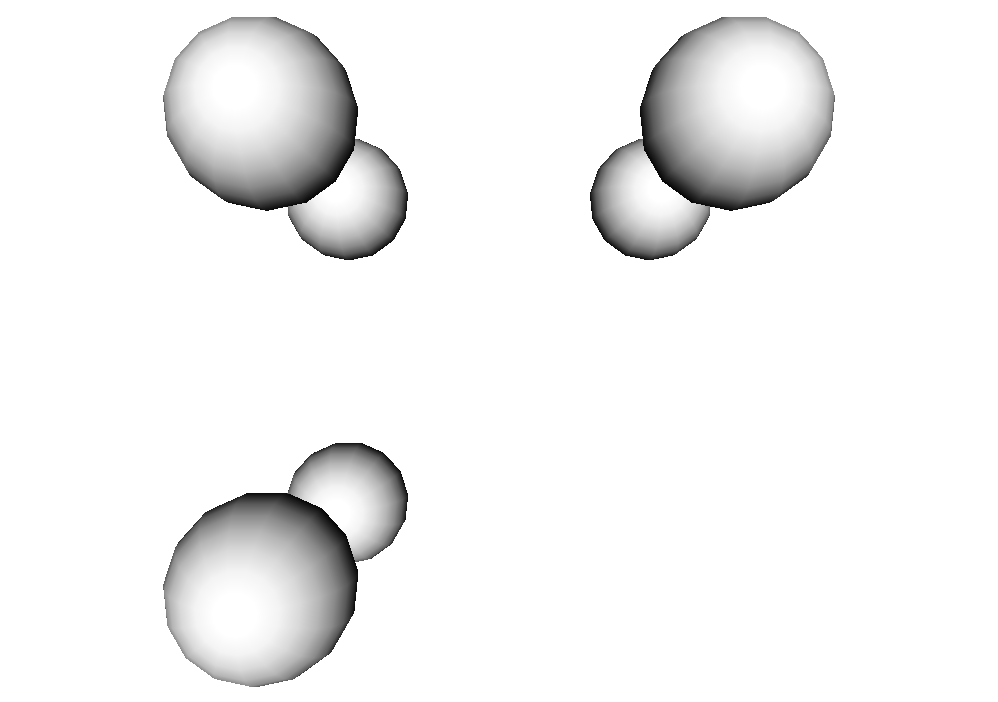
\includegraphics[scale=.3]{images/BCC-incomplete-molecule}
  \caption{\em Cubo BCC incompleto, sin átomo central}
  \label{BCC-incomplete-molecule}
\end{figure}

\begin{figure}[ht]
  \centering
  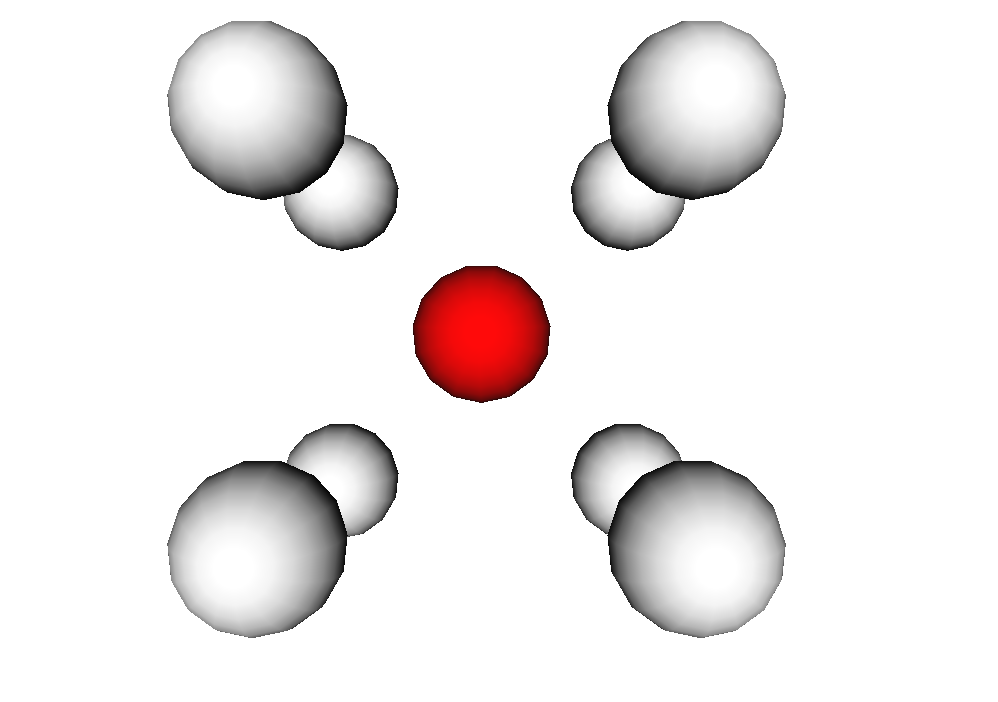
\includegraphics[scale=.3]{images/BCC-complete-molecule}
  \caption{\em Cubo BCC completo, con átomo central}
  \label{BCC-complete-molecule}
\end{figure}

En el caso de los BCC los átomos que conforman la vecindad siempre estarán en las posiciones relativas $[\pm 0.5, \pm 0.5, \pm 0.5]$, es decir, cada átomo puede tener una vecindad compuesta por hasta 8 átomos.

\subsubsection{FCC}
FCC es la clase que maneja los cubos centrados en las caras (\emph{Face Centered Cubic} o \emph{FCC}), los cuales se caracterizan por tener un átomo extra por cara además de uno en cada uno de sus vértices, por lo que además de tener que crear una capa intermedia es necesario modificar la capa primaria, es decir, la que crea el usuario usando el mapa de bits. La regla para agregar estos átomos en las caras es que ellos estén en la diagonal creada por otros 2 átomos, en cualquier dirección. En la figura \ref{FCC-diagonal} se ve como en una estructura cúbica de 1x2, como en una de sus caras se forma una diagonal entre 2 átomos y por lo tanto es necesario agregar un átomo extra en una capa intermedia.

\begin{figure}[ht]
  \centering
  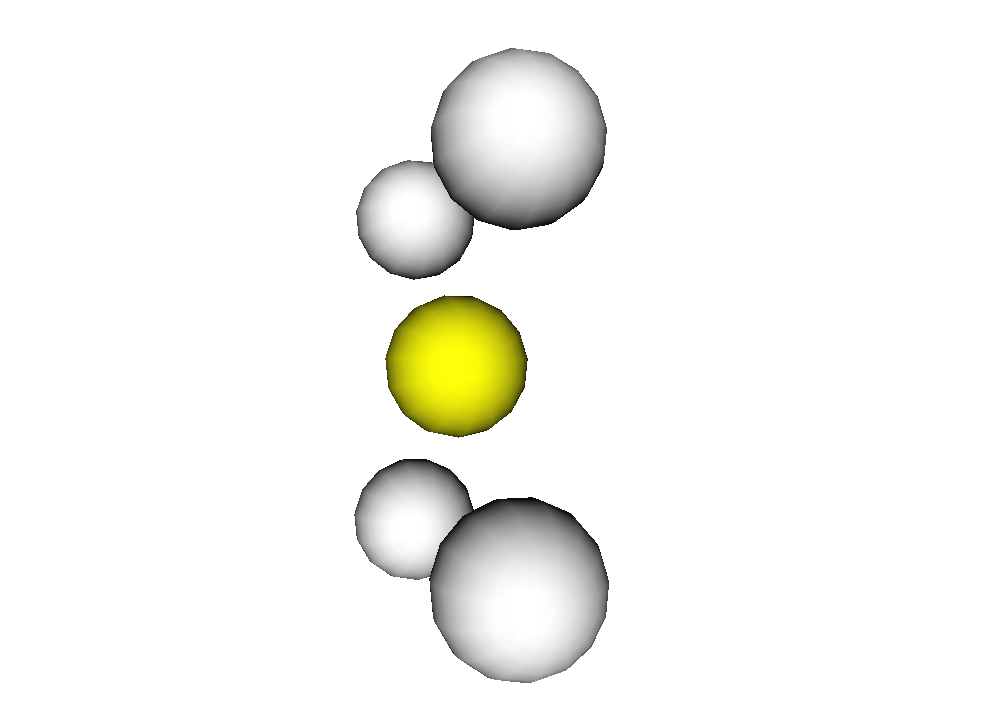
\includegraphics[scale=.3]{images/FCC-diagonal}
  \caption{\em Estructura cúbica FCC, con átomo en una de sus caras}
  \label{FCC-diagonal}
\end{figure}

La vecindad de estas estructuras cúbicas está dada por la posición relativa dada por $[\alpha, \beta, \gamma]$, donde:

\[
	\begin{cases}
		$$(\alpha = \pm 0.5; \beta = \pm 0.5; \gamma = 0)$$ \\
		$$(\alpha = \pm 0.5; \beta = 0; \gamma = \pm 0.5)$$ \\
		$$(\alpha = 0; \beta = \pm 0.5; \gamma = \pm 0.5)$$
	\end{cases}
\]

Lo que resulta en 12 posiciones posibles, siendo este el número máximo de átomos en una vecindad.

\section{Diseño de configuraciones atómicas}

\label{section:disenoConfiguraciones}


El diagrama presentado en la figura \ref{fig:DiagramaSecuenciaDiseno} representa el proceso de diseño de configuraciones atómicas. Para comenzar es necesario definir los parámetros físicos de la configuración, como el tipo de estructura cristalina o la constante de red, y la primera capa de la configuración, en base a un mapa binario de bits. Estas dos acciones no deben ser ejecutadas en un orden en específico, pero ambas son necesarias para el resto de las acciones.

Una vez configurada la configuración a diseñar es posible previsualizarla en 3D, para esto el usuario debe ejecutar una acción (presionar un botón), la que es manejada por un objeto de \emph{LatticeDesigner}, para luego decidir si se debe crear una instancia de \emph{SC}; \emph{BCC} o \emph{FCC}, dependiendo del tipo de estructura cristalina elegida. En la instancia de cubo correspondiente se llama al método \emph{calculate}, el que identifica todos los átomos que pertenecen a la configuración atómica que se está diseñando. Esta a su vez invoca al método \emph{find\_neighborhood} de la súper clase \emph{Cube} con los parámetros correspondientes al tipo de estructura cristalina, para que identifique la vecindad de cada átomo. Luego se pasan los datos de la configuración atómica a la instancia de la clase \emph{AtomCanvas}, la que crea una visualización en 3D de dicha configuración. Para finalizar, \emph{LatticeDesigner} oculta el mapa de bits binario y muestra el \emph{canvas} 3D con la representación de la configuración.

Dentro de la previsualización de la configuración atómica es posible interactuar con esta, haciendo \emph{zoom} o rotándola. Como es necesario que los ejes coordenados representados por una instancia de la clase \emph{Axes} concuerden con la visualización de la instancia de \emph{AtomCanvas}, cada vez que esta última se actualiza es necesario forzar la actualización de los ejes, a través de la referencia en la instancia de \emph{LatticeDesigner}.

Cuando el usuario desea exportar las imágenes de la configuración atómica diseñada, debe invocar el método \emph{export} presente en las clases \emph{Axes} y \emph{AtomCanvas}, pasando como parámetro el nombre de archivo que debe tener el archivo de salida para cada uno de ellos. Este método funciona prácticamente de la misma manera para ambas clases: obtiene el estado actual de los \emph{canvas} 3D, respetando el acercamiento y las rotaciones, y crea un archivo de imagen con el nombre indicado.

Para la exportación del archivo que define la configuración atómica, y que sirve como entrada para la aplicación que efectúa la simulación Monte Carlo, se identifican los átomos pertenecientes a la configuración atómica diseñada invocando al método \emph{calculate} en la clase de cubo correspondiente (\emph{SC}, \emph{BCC} o \emph{FCC}). Una vez identificados todos los átomos se identifica la vecindad para cada uno de ellos, invocando al método \emph{find\_neighborhood} de la súper clase \emph{Cube}. Luego la instancia de \emph{LatticeDesigner} guarda todos los datos un archivo con el formato que exige la aplicación que ejecuta la simulación Monte Carlo.

\begin{figure}[ht]
  \centering
  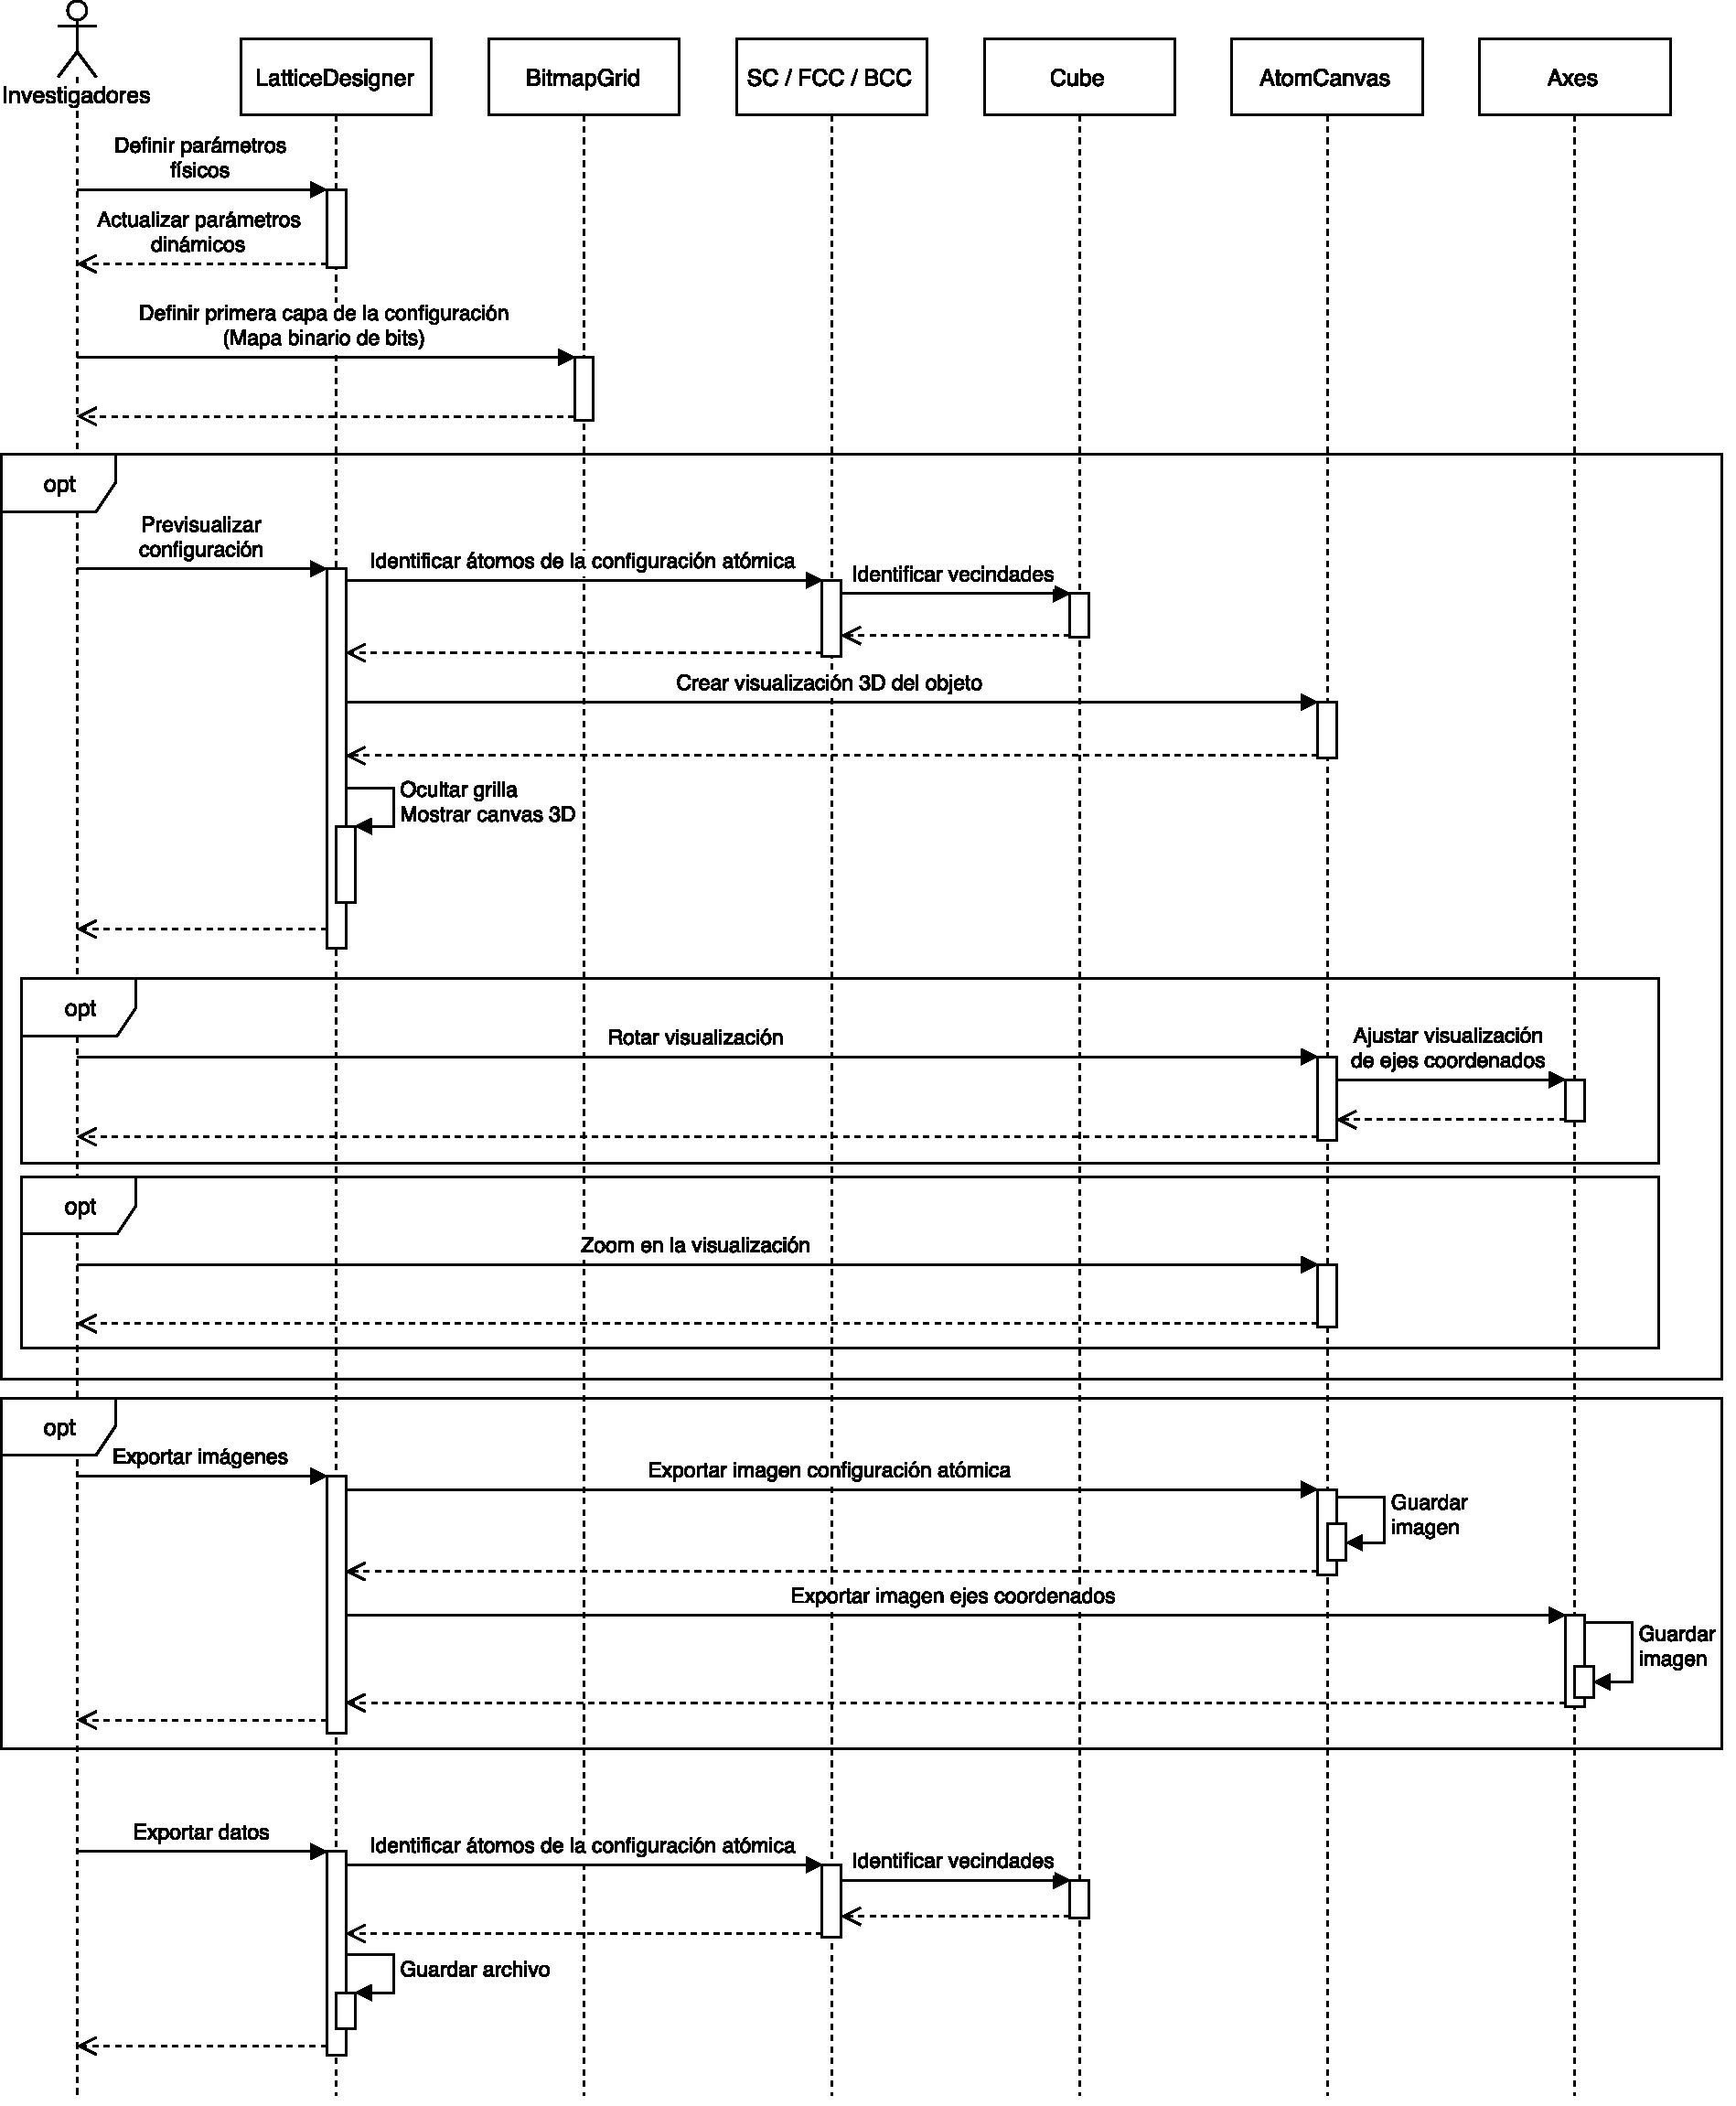
\includegraphics[scale=.5]{images/DiagramaSecuenciaDiseno}
  \caption{\em Diagrama de secuencia para el diseño de una configuración atómica}
  \label{fig:DiagramaSecuenciaDiseno}
\end{figure}

\section{Visualización de resultados de simulación Monte Carlo}

En la figura \ref{fig:DiagramaSecuenciaVisualizacion} se puede ver el diagrama de secuencia del proceso de visualización de resultados de la simulación Monte Carlo. La aplicación que efectúa la simulación genera como resultados un archivo que describe todos los átomos que conforman la configuración atómica. Además por cada $\Delta H$ se genera un archivo con la descripción del vector de magnetización para cada átomo. Para tener una idea, una simulación puede tener más de 2.200 $\Delta H$. Para visualizar los resultados de la simulación es necesario que todos los archivos de salida de la aplicación que la ejecuta se encuentren en el mismo directorio. Además los archivos que describen los vectores de magnetización deben mantener el mismo nombre con que fueron creados.

Para comenzar la visualización es necesario seleccionar el archivo que describe la configuración atómica. Luego la instancia de \emph{LatticeDesigner} valida que los archivos que describen los vectores de magnetización se encuentren en el mismo directorio y valida que todos los archivos sean válidos. Una vez verificado esto se da la opción al usuario de cargar esta información en la memoria para visualizar los resultados. Este proceso se llama ``Carga de archivos de entrada''.

La carga de archivos de entrada consiste en leer cada uno de los archivos que genera la aplicación de simulación Monte Carlo y crear las estructuras de datos necesarias para su visualización. Luego se pasan estos datos a la instancia de \emph{AtomCanvas} para que genere la visualización del 3D de los vectores de magnetización para $t = t_{min}$. Para finalizar se dibuja la curva de histéresis de la simulación, con un marcador que indica que punto de la curva se está representando (ver figura \ref{softwareVisualizacionPlot}).

Dentro del \emph{canvas} 3D es posible la interacción del usuario, tanto de \emph{zoom} como de rotaciones. Estas interacciones son las mismas que en la funcionalidad de ``Diseño de configuraciones atómicas'' y están explicadas en el punto \ref{section:disenoConfiguraciones}.

Dentro de las funcionalidades de la visualización de resultados está el exportar imágenes para publicaciones. Para esto es necesario invocar al método \emph{export} de las instancias de \emph{Axes} y \emph{AtomCanvas}. Esto está explicado en el punto \ref{section:disenoConfiguraciones}. Además es necesario exportar una imagen de la curva de histéresis, indicando el estado actual. Esto se ejecuta directamente en la instancia de \emph{LatticeDesigner}.

Otra de las funcionalidades de la visualización de resultados es el exportar un video con el cambio de estado de los vectores de magnetización a través de toda la simulación, para esto se ejecuta un ciclo para todo $t$ que cumpla con $t_{min} \leq t \leq t_{max}$. Para cada $t$ se actualiza la visualización del resultado en el \emph{canvas} 3D, se obtiene la imagen que representa el estado de los vectores de magnetización y se agrega como un \emph{frame} al video. Una vez obtenidos todos los estados se guarda el archivo de video en la memoria principal.


\begin{figure}[ht]
  \centering
  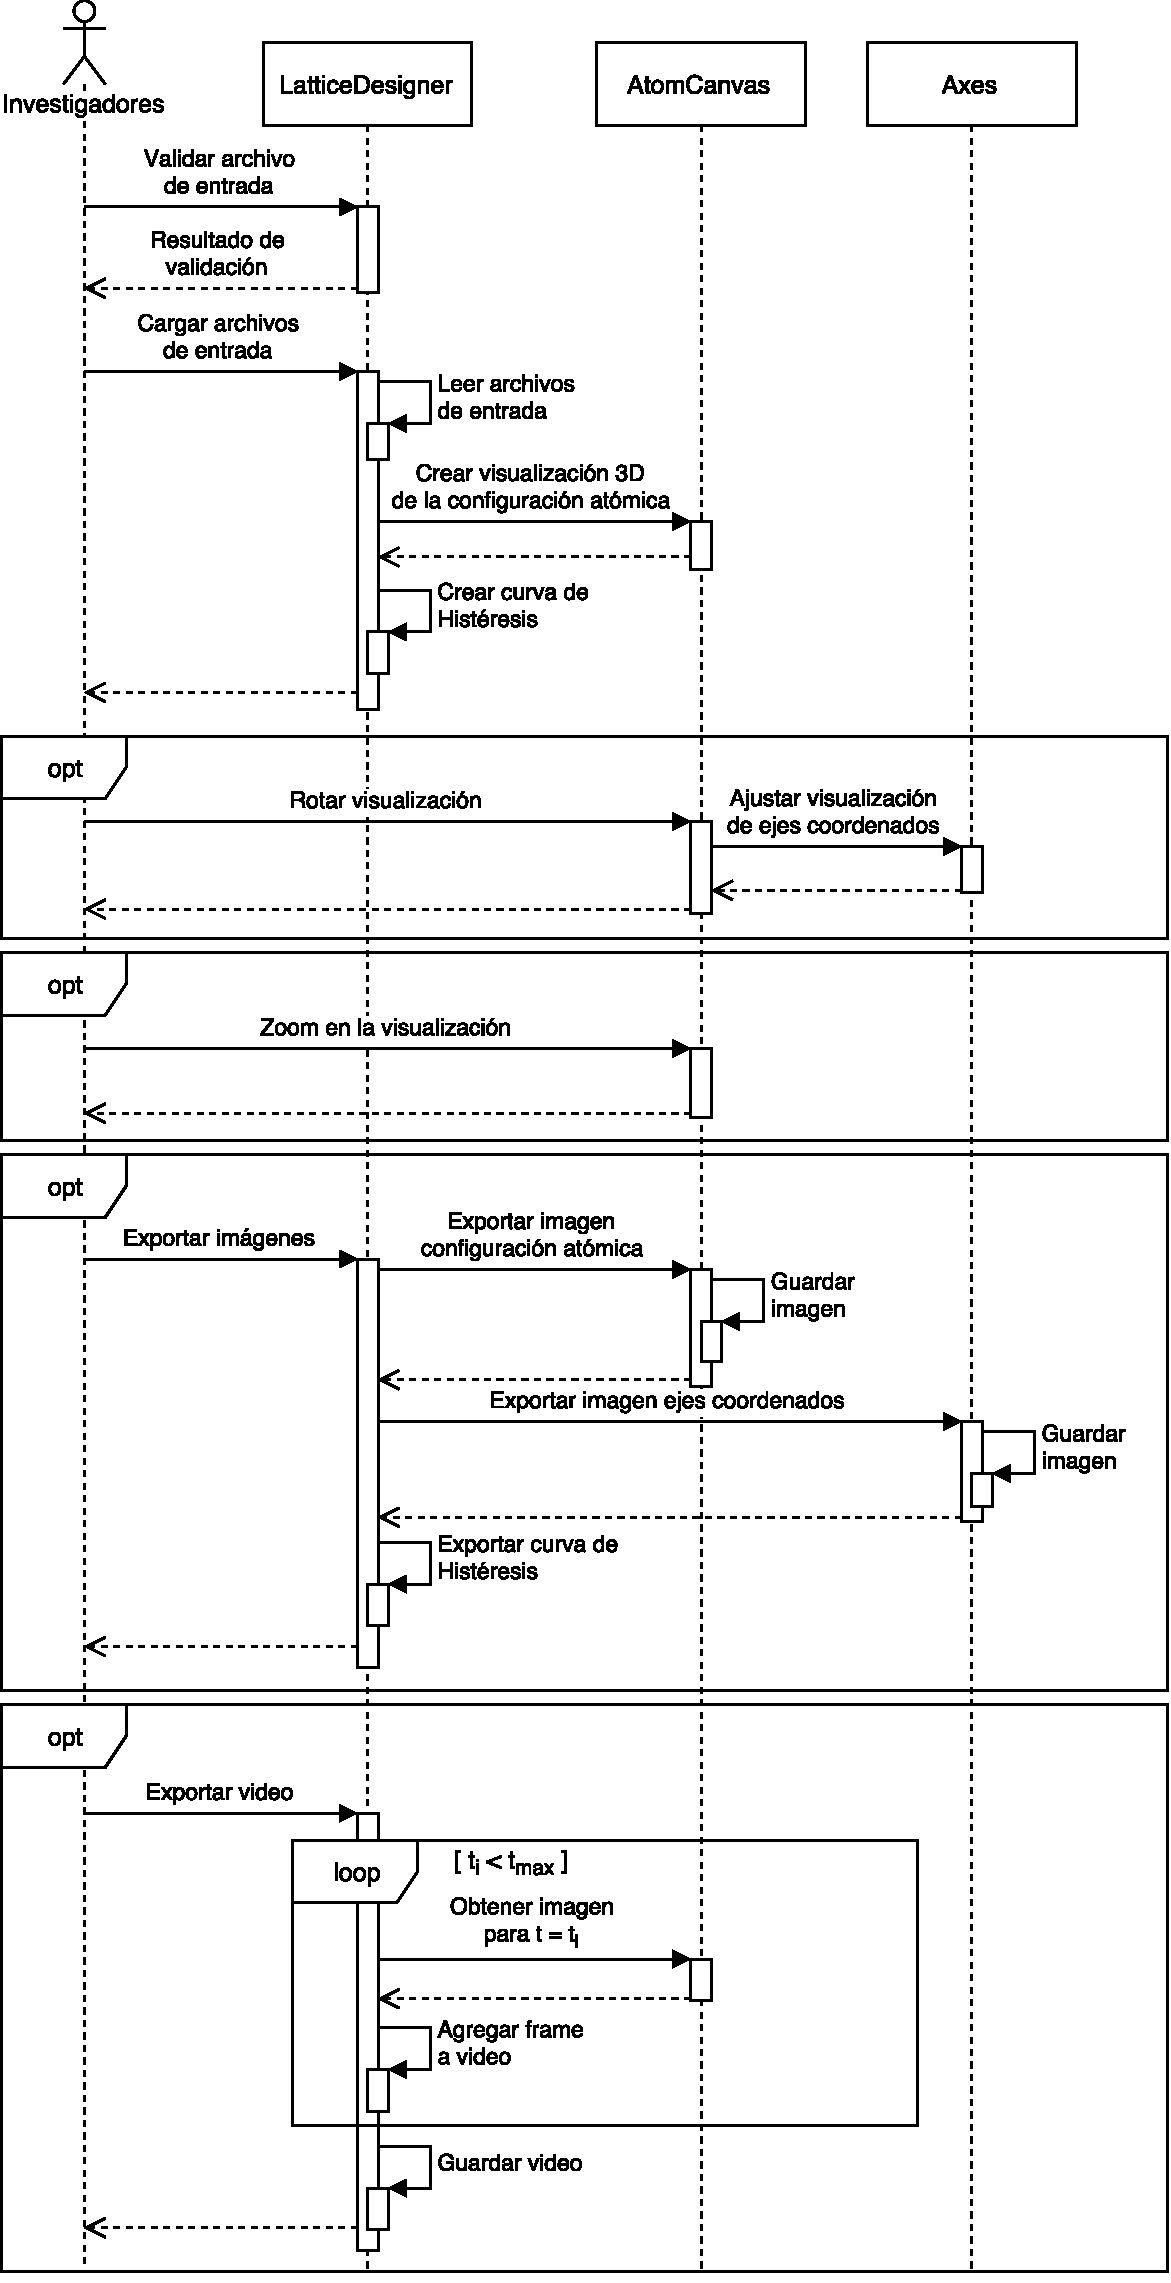
\includegraphics[scale=.5]{images/DiagramaSecuenciaVisualizacion}
  \caption{\em Diagrama de secuencia para la visualización de los resultados de una simulación Monte Carlo}
  \label{fig:DiagramaSecuenciaVisualizacion}
\end{figure}


\section{Identificación de átomos de una configuración}

Para poder generar un archivo que sirva como entrada para la aplicación de la simulación Monte Carlo es necesario determinar todos los átomos que corresponden a la configuración atómica que es diseñaba por un científico. Este proceso, a pesar de tener similitudes, es distinto para cada tipo de estructura cristalina.

Independiente del tipo de estructura cristalina se deben crear tres diccionarios al momento de identificar los átomos que componen la configuración atómica. Estos son: diccionario de átomos; diccionario inverso de átomos y diccionario de tipos de átomos.

\begin{description}
  \item [Diccionario de átomos] \hfill \\
  Este diccionario tiene como llave el ID del átomo y como valor la posicion $[x, y, z]$ del mismo. Se usa para crear la previsualización de la configuración atómica y para crear el archivo que describe la configuración y que es usado para la simulación Monte Carlo.
  \item [Diccionario inverso de átomos] \hfill \\
  Este diccionario tiene como llave las posiciones $x$, $y$ y $z$ de un átomo, separadas por un guión bajo (\_), y como valor el ID del átomo. Por ejemplo para el átomo con ID $15$ en la posición $[1, 2, 3]$ la entrada en el diccionario sería: $[1\_2\_3] \Rightarrow 15$. Este diccionario se usa para buscar la vecindad de cada átomo, ya que se conoce la posición relativa para cada átomo según el tipo de estructura cristalina (ver punto \ref{section:identificacionVecindad}).
  \item [Diccionario de tipo de átomos] \hfill \\
  Este diccionario se usa para seleccionar el color de un átomo en la visualización en 3D de una configuración atómica diseñada. Dependiendo del tipo de estructura cristalina los átomos se pueden categorizar de la siguiente manera:
    \begin{description}
      \item [Átomos de vértice] Son los átomos que están en un vértice de una celda unitaria. Están presentes en todos los tipos de estructura cristalina usados en esta memoria. En la previsualización de una configuración atómica se representan con el color blanco.
      \item [Átomos centrales] Son los átomos que están en el centro de una celda unitaria. Este tipo de átomos se encuentra en las configuraciones atómicas con estructura cristalina BCC. En la previsualización se representan con el color rojo.
      \item [Átomos de cara] Son los átomos que están en una de las caras de una celda unitaria. Este tipo de átomos se encuentra en las configuraciones atómicas con estructura cristalina FCC. En la previsualización se representan con el color amarillo.
    \end{description}
\end{description}

 A continuación se explican los algoritmos usados para cada uno de estos tipos.

\subsection{Cubo simple (SC)}

\label{identificacionAtomosSC}

Para el caso de cubo simple la capa principal debe ser simplemente replicada $n$ veces, donde $n$ es la cantidad de capas que tiene la configuración (ver punto \ref{structureSC}). El estado del mapa de bits binario se guarda en una matriz bidimensional, donde cada casilla marcada se representa con un $1$. Se recorre esta matriz buscando todas las casillas marcadas, de tal forma de obtener la capa primaria que será replicada. En un arreglo unidimensional se guarda una tupla de tipo $(x, y)$ para cada casilla marcada. Esto se puede ver en el algoritmo \ref{alg:TopLayerSC}.

\begin{algorithm}[ht]
  \caption{Obtener capa primaria para estructuras cristalinas}
  \label{alg:TopLayerSC}
  \begin{algorithmic}[1]
    \FOR {$i = 1$ \TO $Ancho\ grilla$}
      \FOR {$j = 1$ \TO $Alto\ grilla$}
        \IF {$Grilla[i][j] == 1$}
          \STATE Agregar a $CapaPrimaria$ = $(i, j)$
        \ENDIF
      \ENDFOR
    \ENDFOR
  \end{algorithmic}
\end{algorithm}

Luego necesitamos agregar la componente $z$ para cada capa de la configuración atómica, obteniendo la posición final de cada átomo. Para esto se ejecuta un ciclo $n$ veces, donde $n$ es la cantidad de capas que tiene la configuración. Finalmente, cuando se tiene la posición de cada átomo, se agrega a cada uno de los 3 diccionarios necesarios (Ver algoritmo \ref{alg:identifyAtomsSC}).

\begin{algorithm}[ht]
  \caption{Identificar átomos para estructura cristalina de tipo SC}
  \label{alg:identifyAtomsSC}
  \begin{algorithmic}[1]
    \STATE $ID\ atomo \leftarrow 1$
    \FOR {$z = 1$ \TO $Numero\ de\ capas$}
      \FOR {cada posición $(x, y)$ en $CapaPrimaria$}
        \STATE $atomos[ID\ atomo] \leftarrow (x, y, z)$
        \STATE $atomos\_por\_posicion[x\_y\_z] \leftarrow ID\ atomo$
        \STATE $tipo\_de\_atomo[ID\ atomo] \leftarrow Vertice$
        \STATE $ID\ atomo \leftarrow ID\ atomo + 1$
      \ENDFOR
    \ENDFOR
  \end{algorithmic}
\end{algorithm}

Cabe notar que para una configuración atómica con estructura cristalina de tipo SC todos los átomos serán de tipo ``Vértice''.

\subsection{Cubo centrado en el cuerpo (BCC)}

\label{identifyAtomsBCC}

Para las estructuras cristalinas de tipo BCC es necesario hacer algunas modificaciones al algoritmo usado para el cubo simple. En este caso también debemos obtener la capa primaria usando el algoritmo \ref{alg:TopLayerSC}. Además debemos obtener la capa intermedia, que contendrá todos los átomos centrales del cubo. Tal como está explicado en el punto \ref{structureBCC} es necesario que existan los 4 átomos de vértice en una celda unitaria para agregar el átomo central. Para esto se usará el algoritmo \ref{alg:IntermediateLayerBCC}.

\begin{algorithm}[ht]
  \caption{Obtener capa intermedia para estructura cristalina de tipo BCC}
  \label{alg:IntermediateLayerBCC}
  \begin{algorithmic}[1]
    \FOR {$i = 1$ \TO $Ancho\ grilla$}
      \FOR {$j = 1$ \TO $Alto\ grilla$}
        \IF {$Grilla[i][j] == 1$ y $Grilla[i+1][j] == 1$ y $Grilla[i][j+1] == 1$ y $Grilla[i+1][j+1] == 1$}
          \STATE Agregar a $CapaIntermedia$ = $(i + 0.5, j + 0.5)$
        \ENDIF
      \ENDFOR
    \ENDFOR
  \end{algorithmic}
\end{algorithm}

Una vez teniendo la capa primaria y la capa intermedia para la configuración atómica se deben identificar todos los átomos de dicha configuración. Para saber cuantas capas de cada tipo se crearan es necesario dividir el número total de capas en 2. En caso de ser que el número de capas sea impar se usa la aproximación al entero mayor ($ceil()$) para la cantidad de capas primarias y la aproximacion al entero menor ($floor()$) para la cantidad de capas intermedias. Esto se muestra en el algoritmo \ref{alg:identifyAtomsBCC}.

\begin{algorithm}[ht]
  \caption{Identificar átomos para estructura cristalina de tipo BCC}
  \label{alg:identifyAtomsBCC}
  \begin{algorithmic}[1]
    \STATE $ID\ atomo \leftarrow 1$
    \STATE $capas\_primarias = ceil(Numero\ de\ capas)$
    \STATE $capas\_intermedias = floor(Numero\ de\ capas)$
    \FOR {$z = 1$ \TO $capas\_primarias$}
      \FOR {cada posición $(x, y)$ en $CapaPrimaria$}
        \STATE $atomos[ID\ atomo] \leftarrow (x, y, z)$
        \STATE $atomos\_por\_posicion[x\_y\_z] \leftarrow ID\ atomo$
        \STATE $tipo\_de\_atomo[ID\ atomo] \leftarrow Vertice$
        \STATE $ID\ atomo \leftarrow ID\ atomo + 1$
      \ENDFOR
    \ENDFOR
    \FOR {$z = 1$ \TO $capas\_intermedias$}
      \FOR {cada posición $(x, y)$ en $CapaIntermedia$}
        \STATE $zReal \leftarrow z + 0.5$
        \STATE $atomos[ID\ atomo] \leftarrow (x, y, zReal)$
        \STATE $atomos\_por\_posicion[x\_y\_zReal] \leftarrow ID\ atomo$
        \STATE $tipo\_de\_atomo[ID\ atomo] \leftarrow Central$
        \STATE $ID\ atomo \leftarrow ID\ atomo + 1$
      \ENDFOR
    \ENDFOR
  \end{algorithmic}
\end{algorithm}

\subsection{Cubo centrado en sus caras (FCC)}

Para los cubos centrados en sus caras es necesario crear 3 tipos de capas:
\begin{description}
  \item[Capa primaria] Esta capa define los átomos en los vértices de las capas primarias. Es la misma capa que se usa para las estructuras cristalinas SC y BCC. Para obtener esta capa se usa el algoritmo \ref{alg:TopLayerSC}.
  \item[Capa de cara primaria] Esta capa define los átomos de cara que están a la misma altura que los de la Capa Primaria.
  \item[Capa de cara intermedia] Esta capa define los átomos de cara que están entre 2 capas primarias.
\end{description}

Tal como se describe en el punto \ref{structureFCC}, un átomo de cara se crea cuando este está sobre una diagonal formada por 2 átomos de vértice. Esto se obtiene usando el algoritmo \ref{alg:FaceLayersFCC}. Como se puede notar, en algunos casos este algoritmo puede definir un átomo de cara más de una vez, por lo que luego de ser ejecutado es necesario buscar todas las tuplas repetidas para cada una de las matrices.

\begin{algorithm}[ht]
  \caption{Obtener capas de cara para estructura cristalina de tipo FCC}
  \label{alg:FaceLayersFCC}
  \begin{algorithmic}[1]
    \FOR {$i = 1$ \TO $Ancho\ grilla$}
      \FOR {$j = 1$ \TO $Alto\ grilla$}
        \IF {$Grilla[i+1][j+1] == 1$}
          \STATE Agregar a $CapaCaraPrimaria$ = $(i + 0.5, j + 0.5)$
        \ENDIF
        \IF {$Grilla[i+1][j-1] == 1$}
          \STATE Agregar a $CapaCaraPrimaria$ = $(i i 0.5, j - 0.5)$
        \ENDIF
        \IF {$Grilla[i][j+1] == 1$}
          \STATE Agregar a $CapaCaraIntermedia$ = $(i, j + 0.5)$
        \ENDIF
        \IF {$Grilla[i+1][j] == 1$}
          \STATE Agregar a $CapaCaraIntermedia$ = $(i + 0.5, j)$
        \ENDIF
      \ENDFOR
    \ENDFOR
  \end{algorithmic}
\end{algorithm}

Una vez que se tienen las 3 capas necesarias se usa el algoritmo \ref{alg:identifyAtomsFCC} para identificar los átomos de la configuración cristalina. Este algoritmo es muy similar al usado para identificar los átomos de unan estructura cristalina de tipo BCC (ver algoritmo \ref{alg:identifyAtomsBCC}). Ambos difieren en que al definir los átomos de las capas primarias es necesario tomar en cuenta tanto los átomos de la matriz $CapaPrimaria$ como los de la matriz $CapaCaraPrimaria$ para las estructuras cristalinas de tipo FCC.

\begin{algorithm}[ht]
  \caption{Identificar átomos para estructura cristalina de tipo FCC}
  \label{alg:identifyAtomsFCC}
  \begin{algorithmic}[1]
    \STATE $ID\ atomo \leftarrow 1$
    \STATE $capas\_primarias = ceil(Numero\ de\ capas)$
    \STATE $capas\_intermedias = floor(Numero\ de\ capas)$
    \FOR {$z = 1$ a $capas\_primarias$}
      \FOR {cada posición $(x, y)$ en $CapaPrimaria$}
        \STATE $atomos[ID\ atomo] \leftarrow (x, y, z)$
        \STATE $atomos\_por\_posicion[x\_y\_z] \leftarrow ID\ atomo$
        \STATE $tipo\_de\_atomo[ID\ atomo] \leftarrow Vertice$
        \STATE $ID\ atomo \leftarrow ID\ atomo + 1$
      \ENDFOR
      \FOR {cada posición $(x, y)$ en $CapaCaraPrimaria$}
        \STATE $atomos[ID\ atomo] \leftarrow (x, y, z)$
        \STATE $atomos\_por\_posicion[x\_y\_z] \leftarrow ID\ atomo$
        \STATE $tipo\_de\_atomo[ID\ atomo] \leftarrow Vertice$
        \STATE $ID\ atomo \leftarrow ID\ atomo + 1$
      \ENDFOR
    \ENDFOR
    \FOR {$z = 1$ a $capas\_intermedias$}
      \FOR {cada posición $(x, y)$ en $CapaCaraIntermedia$}
        \STATE $zReal \leftarrow z + 0.5$
        \STATE $atomos[ID\ atomo] \leftarrow (x, y, zReal)$
        \STATE $atomos\_por\_posicion[x\_y\_zReal] \leftarrow ID\ atomo$
        \STATE $tipo\_de\_atomo[ID\ atomo] \leftarrow Central$
        \STATE $ID\ atomo \leftarrow ID\ atomo + 1$
      \ENDFOR
    \ENDFOR
  \end{algorithmic}
\end{algorithm}

\section{Identificación de vecindad para un átomo}
\label{section:identificacionVecindad}

Cuando se diseña una configuración atómica es necesario identificar los vecinos más cercanos para cada átomo. Debido a que el algoritmo de búsqueda es similar para los tres tipos de estructuras cristalinas, este se efectúa en la clase \emph{Cube}, padre de las clases \emph{SC}, \emph{BCC} y \emph{FCC}.

Para identificar la vecindad de cada átomo se usa el diccionario inverso de átomos creado en la etapa de identificación de átomos (ver punto \ref{identificacionAtomosSC}). Según el tipo de estructura cristalina se pueden identificar las distintas posiciones relativas de los vecinos en un átomo.

Por ejemplo, para un átomo en una estructura cristalina de tipo SC se sabe que los vecinos se encuentran en las posiciones relativas $[-1,0,0]$, $[1,0,0]$, $[0,-1,0]$, $[0,1,0]$, $[0,0,-1]$ y $[0,0,1]$ (más información en los puntos \ref{structureSC} y \ref{cubeClasesSC}). Por lo tanto para un átomo en la posición $[1, 2, 3]$ sus vecinos pueden estar en las siguientes ubicaciones:

\begin{itemize}
  \item $[1, 2, 3] + [-1, 0, 0] = [0, 2, 3]$
  \item $[1, 2, 3] + [1, 0, 0] = [2, 2, 3]$
  \item $[1, 2, 3] + [0, -1, 0] = [1, -1, 3]$
  \item $[1, 2, 3] + [0, 1, 0] = [1, 3, 3]$
  \item $[1, 2, 3] + [0, 0, -1] = [1, 2, 2]$
  \item $[1, 2, 3] + [0, 0, 1] = [1, 2, 4]$
\end{itemize}

Luego se deben buscar, en el diccionario inverso de átomos, las siguientes llaves: ``0\_2\_3'', ``2\_2\_3'', ``1\_-1\_3'', ``1\_3\_3'', ``1\_2\_2'' y ``1\_2\_4''.

Este proceso se puede ver en el algoritmo \ref{alg:findNeighborhood}.

Desde el método \emph{find\_neighborhood} en las clases \emph{SC}, \emph{BCC} y \emph{FCC} se invoca al método de la súper clase \emph{Cubes} con las siguientes posiciones relativas por tipo de estructura cristalina:

\begin{description}
  \item [Cubo simple] $[-1,0,0]$, $[1,0,0]$, $[0,-1,0]$, $[0,1,0]$, $[0,0,-1]$ y $[0,0,1]$.
  \item [Cubo centrado en su cuerpo] $[0.5, 0.5, 0.5]$, $[0.5, -0.5, 0.5]$, $[-0.5, 0.5, 0.5]$, $[-0.5, -0.5, 0.5]$, $[0.5, 0.5, -0.5]$, $[0.5, -0.5, -0.5]$, $[-0.5, 0.5, -0.5]$ y $[-0.5, -0.5, -0.5]$.
  \item [Cubo centrado en sus caras] $[0, 0.5, 0.5]$, $[0, 0.5, -0.5]$, $[0, -0.5, 0.5]$, $[0, -0.5, -0.5]$, $[0.5, 0, 0.5]$, $[0.5, 0, -0.5]$, $[-0.5, 0, 0.5]$, $[-0.5, 0, -0.5]$, $[0.5, 0.5, 0]$, $[0.5, -0.5, 0]$, $[-0.5, 0.5, 0]$ y $[-0.5, -0.5, 0]$.
\end{description}

\begin{algorithm}[ht]
  \caption{Obtener los vecinos de átomos en base a posiciones relativas}
  \label{alg:findNeighborhood}
  \begin{algorithmic}[1]
    \STATE $vecinos = \{\ \}$ \COMMENT{Diccionario vacío}
    \FORALL {$ID\ atomo, posicionAtomo$ en $Atomos$}
      \STATE $vecinosAtomo = [\ ]$ \COMMENT{Matriz vacía}
      \FORALL {$posicionVecino$ en $posicionesVecinos$}
        \STATE $posicionDondeBuscar \leftarrow posicionAtomo + posicionVecino$
        \IF {existe llave $posicionDondeBuscar$ en $diccionarioInverso$}
          \STATE $ID\ Vecino \leftarrow diccionarioInverso[posicionDondeBuscar]$
          \STATE Agregar a $vecinosAtomo$ = $ID Vecino$
        \ENDIF
      \ENDFOR
      \STATE $vecinos[ID\ atomo] \leftarrow vecinos$
    \ENDFOR
  \end{algorithmic}
\end{algorithm}







